\documentclass{article}
\usepackage{graphicx} % Required for inserting images
\usepackage[left=4cm, right=4cm, top=4cm, bottom=4cm]{geometry}
\usepackage[T1]{fontenc}
\usepackage[polish]{babel}
\usepackage{amssymb}
\usepackage{url}
\usepackage{enumitem}
\usepackage{dirtree}
\usepackage[export]{adjustbox}
\usepackage{amsmath}
\usepackage{float}




\title{\Huge JIMP2 Projekt 2025 \\ {\huge Dokumentacja końcowa - Java}}
\author{Michał Ludwiczak \\ GR3}
\date{10 czerwca 2025}

\begin{document}

\maketitle

\tableofcontents


\begin{figure} [H]
    \centering
    
\includegraphics[width=0.5\linewidth]{img/icon_dark.png}
    \caption{Ikona / Logo programu}
    \label{fig:icon_dark}
\end{figure}



\section{Cel projektu}

    Cel projektu to stworzenie aplikacji w języku Java, umożliwiającej podział grafu na określoną przez użytkownika liczbę części, z zachowaniem określonego lub domyślnego 10-procentowego marginesu różnicy liczby wierzchołków pomiędzy częściami. Domyślnie graf dzielony jest na dwie części. Celem podziału jest także minimalizacja liczby przeciętych krawędzi pomiędzy powstałymi częściami grafu. 
    Aplikacja ma być wyposażona w graficzny interfejs użytkownika wykonany w technologii Swing. Użytkownik będzie mógł wczytywać już podzielony graf z pliku tekstowego lub binarnego, wczytywać niepodzielone grafy, definiować liczbę części oraz margines podziału, a także zapisywać wynikowy graf wraz z danymi wejściowymi do pliku tekstowego lub binarnego. 
    Każda część grafu będzie prezentowana w interfejsie graficznym w odrębnym kolorze.
    
    \begin{figure}[H]
        \centering
        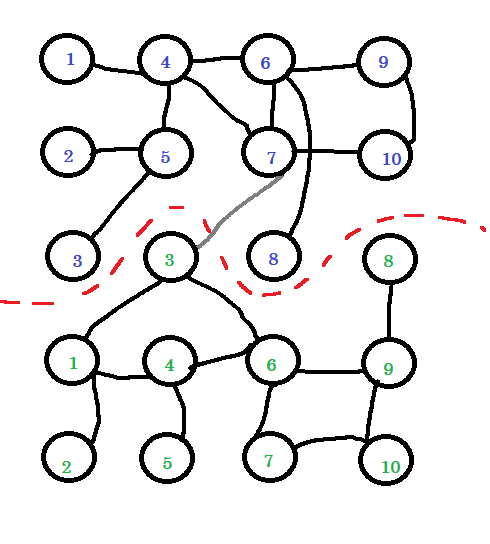
\includegraphics[width=0.75\linewidth]{img/graph.png}
        \caption{Przykładowy graf podzielony na 2 równe części}
        \label{fig:graph}
    \end{figure}



\section{Problem}

    Podział grafu na części w taki sposób, aby liczba przeciętych krawędzi była jak najmniejsza, nie jest problemem łatwym. Znalezienie optymalnego rozwiązania dla dużych grafów jest praktycznie niewykonalne w rozsądnym czasie, ponieważ liczba możliwych podziałów rośnie wykładniczo wraz z liczbą wierzchołków.
    W przypadku podziału grafu na dwie części istnieje \( 2^{n-1} - 1 \) możliwych sposobów podziału, gdzie \( n \) oznacza liczbę wierzchołków. Z tego powodu zamiast sprawdzania wszystkich możliwych podziałów stosuje się algorytmy przybliżone, heurystyki lub algorytmy zachłanne, które pozwalają na szybkie znalezienie dobrego, choć niekoniecznie optymalnego rozwiązania.

\section{Algorytm}

W programie zdecydowałem się użyć metody spektralnej dzielenia grafu, która wykorzystuje własności spektralne macierzy Laplace'a grafu. Na podstawie spektrum grafu, które opisuje jego strukturę graf możemy podzielić w efektywny i satysfakcjonujący sposób, minimalizując liczbę przeciętych krawędzi.


    \subsection{Macierz Laplace'a}
    
    W podejściu spektralnym do podziału grafu kluczową rolę odgrywa macierz Laplace'a \cite{laplacian_matrix}.
    Wzór na Laplacian klasyczny definiuje się jako:
    \[
    \mathbf{L} = \mathbf{D} - \mathbf{A}
    \]
    gdzie:
    \begin{itemize}
      \item \( L \) to \textbf{macierz Laplace'a} grafu,
      \item \( D \) to \textbf{macierz stopni} to macierz diagonalna, w której elementy na diagonali \( d_{ii} \) odpowiadają stopniowi wierzchołka \( i \), czyli liczbie krawędzi, które są z nim bezpośrednio połączone. W przypadku pętli, każda taka krawędź zwiększa stopień wierzchołka o 2, ponieważ jest traktowana jako dwie krawędzie incydentne z tym samym wierzchołkiem
      \item \( A \) to \textbf{macierz sąsiedztwa} grafu, gdzie elementy \( a_{ij} \) są równe 1, jeśli istnieje krawędź między wierzchołkami \( i \) i \( j \), oraz 0 w przeciwnym przypadku.
    \end{itemize}

    

    \subsection{Obliczenie par własnych}

    Następnym krokiem jest obliczenie \(k = p - 1\) (gdzie \(p\) to liczba części, na które graf ma być podzielony) najmniejszych wektorów własnych, z których pierwszy zerowy zostanie pominięty. Dla bisekcji będzie to jeden wektor, tzw. drugi najmniejszy – wektor Fiedlera. Wektory własne macierzy Laplace'a grafu przechowują informacje o połączeniach pomiędzy wierzchołkami.
    
    Do obliczenia tych par własnych wykorzystano bibliotekę ARPACK (poprzez binding Java: \texttt{com.github.fommil.netlib.ARPACK}), która implementuje metodę Implicitly Restarted Lanczos Method (IRLM) – specjalizowaną wersję metody Arnoldiego dla macierzy symetrycznych. ARPACK wymaga jedynie implementacji mnożenia macierzy przez wektor, co pozwala na efektywne wykorzystanie pamięci proporcjonalnie do liczby niezerowych elementów macierzy (format CSR). Dzięki temu rozwiązanie dobrze sprawdza się przy analizie dużych, rzadkich grafów.



    \subsection{Podział}

    \subsubsection{Podział według wektora Fiedlera}
    
    Podział grafu według wektora Fiedlera polega na wykorzystaniu drugiego najmniejszego wektora własnego macierzy Laplasjanu grafu, nazywanego wektorem Fiedlera. Ten wektor koduje informację o strukturze spójności grafu – wierzchołki o podobnych wartościach współrzędnych tego wektora leżą blisko siebie w grafie. W implementacji sortuje się wierzchołki według wartości wektora Fiedlera i dzieli na dwie grupy o równej liczności.
    
    \subsubsection{Klasteryzacja}
    Po otrzymaniu macierzy zawierającej \(k\) wektorów własnych (gdzie \(k = p\)), każdy wierzchołek grafu jest reprezentowany jako punkt w \(k\)-wymiarowej przestrzeni. W celu podziału grafu na \(p\) części, zastosowano algorytm centroidów (k-means) \cite{k-means}. Centroidy są inicjalizowane równomiernie wzdłuż głównych osi na podstawie zakresu wartości współrzędnych. Następnie iteracyjnie przypisuje się wierzchołki do najbliższych centroidów, z zachowaniem ograniczenia liczebności każdego klastra (tak, aby podziały były możliwie równe). Po każdej iteracji aktualizowane są położenia centroidów na podstawie średniej pozycji przypisanych punktów. Proces powtarzany jest do momentu osiągnięcia zbieżności (braku zmian centroidów) lub osiągnięcia maksymalnej liczby iteracji.



    \subsection{Wynik}

    Po otrzymaniu poszczególnych części z wierzchołkami modyfikuje się macierz sąsiedztwa \(A\) w formacie CSR usuwając krawędzie pomiędzy wierzchołkami przynależącymi do różnych grup. W ten sposób otrzymuje się nową macierz sąsiedztwa, która zawiera już podzielony graf. Macierz sąsiedztwa jest już gotowa do przetworzenia i wypisania na plik wyjściowy.
    


\section{Interfejs graficzny}

    Aplikacja została zaprojektowana z wykorzystaniem biblioteki Swing i oferuje graficzny interfejs użytkownika, który umożliwia interaktywną obsługę procesu podziału grafu.

    \begin{figure}[H]
        \centering
        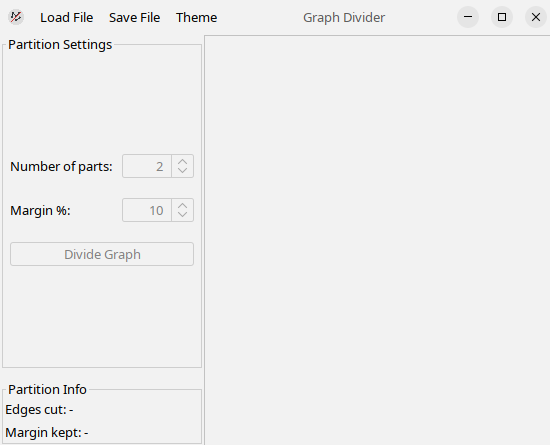
\includegraphics[width=1\linewidth]{img/gui.png}
        \caption{Interfejs programu GraphDivider}
        \label{fig:gui}
    \end{figure}


    Główne okno aplikacji składa się z:
    
    \begin{itemize}
    
        \item \textbf{Paska menu}, który umożliwia:
        \begin{itemize}
            \item wybranie pliku z grafem do wczytania:
            \begin{itemize}
                \item niepodzielony graf w formacie tekstowym,
                \item podzielony graf w formacie tekstowym,
                \item podzielony graf w formacie binarnym
            \end{itemize}
            \begin{figure}[H]
                \centering
                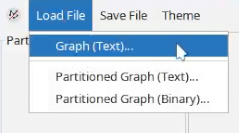
\includegraphics[width=0.5\linewidth]{img/load_file.png}
                \caption{Opcja wczytania pliku}
                \label{fig:load_file}
            \end{figure}
            
            \item zapisanie pliku z podzielonym grafem w formacie:
            \begin{itemize}
                \item tekstowym,
                \item binarnym
            \end{itemize}
            \begin{figure}[H]
                \centering
                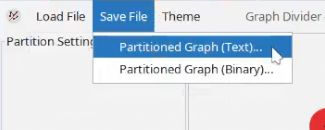
\includegraphics[width=0.5\linewidth]{img/save_file.png}
                \caption{Opcja zapisu pliku}
                \label{fig:save_file}
            \end{figure}
            
            \item zmianę motywu:
            \begin{itemize}
                \item automatyczny / systemowy,
                \item jasny,
                \item ciemny
            \end{itemize}
            \begin{figure}[H]
                \centering
                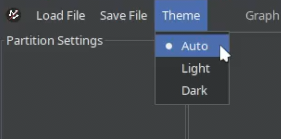
\includegraphics[width=0.5\linewidth]{img/theme.png}
                \caption{Opcja motywu}
                \label{fig:theme}
            \end{figure}
        \end{itemize}
        
        \item \textbf{Bocznego panelu podziału}, który umożliwia wybranie liczby części oraz marginesu podziału, a także rozpoczęcie podziału.

        \begin{figure}[H]
            \centering
            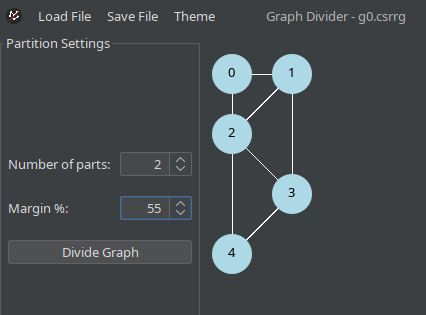
\includegraphics[width=0.75\linewidth]{img/tool_panel.png}
            \caption{Boczny panel podziału}
            \label{fig:tool_panel}
        \end{figure}
        
        \item \textbf{Panelu informacji}, który wyświetla liczbę przeciętych krawędzi i zachowany margines po podziale.

        \begin{figure}[H]
            \centering
            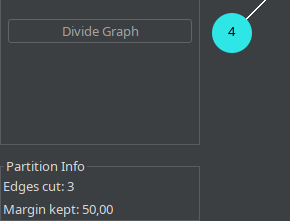
\includegraphics[width=0.75\linewidth]{img/info.png}
            \caption{Panel informacji o podziale}
            \label{fig:info}
        \end{figure}

        \item \textbf{Panelu grafu}, który wyświetla zarówno graf przed podzieleniem, jak i po podzieleniu kolorując poszczególne podgrafy.

        \begin{figure}[H]
            \centering
            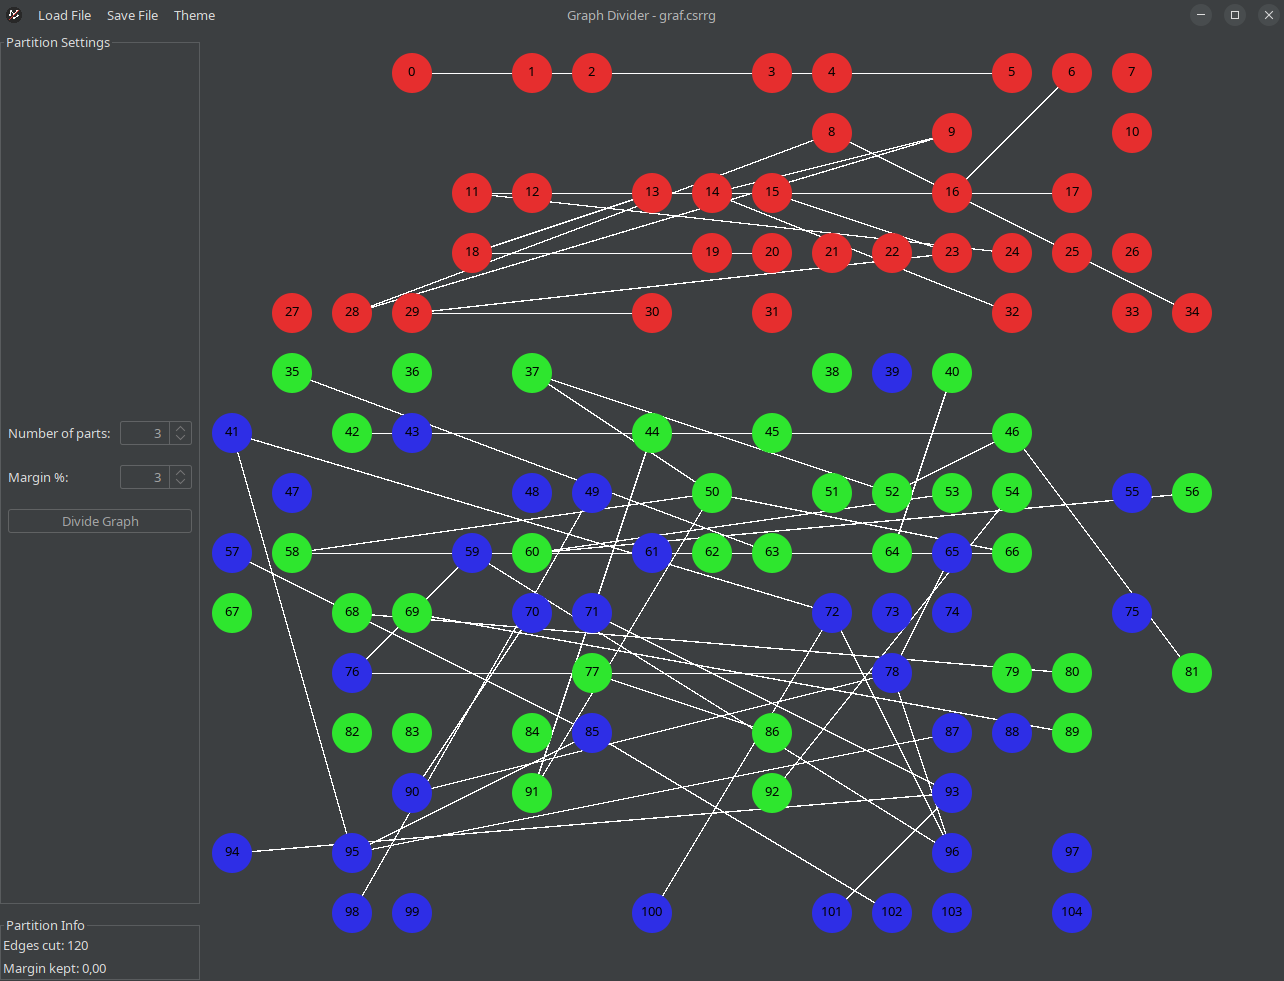
\includegraphics[width=1\linewidth]{img/graphpanel.png}
            \caption{Panel grafu (po podziale)}
            \label{fig:graph}
        \end{figure}
        
    \end{itemize}



\section{Struktura projektu}

    Projekt korzysta z systemu budowania Gradle. Wszystkie zależności oraz zadania budowania są zdefiniowane w pliku \texttt{build.gradle}. Do kompilacji i uruchamiania aplikacji wystarczy użyć poleceń \texttt{./gradlew build} / \texttt{gradle build} oraz \texttt{./gradlew run} / \texttt{gradle run}. Do poprawnej kompilacji i uruchomienia projektu wymagane jest również środowisko Java Development Kit (JDK) w wersji co najmniej 21.

    Projekt został zorganizowany w następujący sposób:

    \begin{itemize}
        \item \texttt{build.gradle} -- główny plik konfiguracyjny Gradle, definiuje zależności i zadania budowania projektu.
        \item \texttt{settings.gradle} -- plik ustawień projektu Gradle.
        \item \texttt{gradlew}, \texttt{gradlew.bat}, \texttt{gradle/wrapper/} -- skrypty i pliki wrappera Gradle, umożliwiające budowanie projektu bez konieczności instalowania Gradle globalnie.
        \item \texttt{build/} -- katalog generowany automatycznie przez Gradle, zawiera artefakty kompilacji.
        \item \texttt{docs/} -- dokumentacja projektu (funkcjonalna, implementacyjna, diagramy UML).
        \item \texttt{src/main/java/graphdivider/} -- główny kod źródłowy aplikacji:
        \begin{itemize}
            \item \texttt{Main.java} -- klasa uruchamiająca aplikację.
            \item \texttt{controller/} -- logika sterująca aplikacją.
            \item \texttt{io/} -- obsługa wejścia/wyjścia (wczytywanie i zapisywanie plików).
            \item \texttt{model/} -- klasy modelujące strukturę grafu oraz algorytmy (m.in. macierz Laplace'a, obliczanie par własnych, klasteryzacja).
            \item \texttt{view/} -- klasy odpowiedzialne za interfejs graficzny (Swing).
        \end{itemize}
        \item \texttt{src/main/resources/} -- zasoby aplikacji:
        \begin{itemize}
            \item \texttt{graphs/} -- przykładowe pliki wejściowe z grafami w formacie .csrrg.
            \item \texttt{divided\_graphs/} -- pliki wyjściowe z programu w C z podzielonymi grafami w formacie tekstowym i binarnym.
            \item \texttt{icon/} -- pliki graficzne, ikony.
            \item \texttt{output/} -- katalog na generowane pliki wyjściowe.
        \end{itemize}
    \end{itemize}



\section{Architektura MVC}

W projekcie zastosowano wzorzec architektoniczny \textbf{Model-View-Controller (MVC)}.  
Logika aplikacji została podzielona na trzy główne warstwy:

\begin{itemize}
    \item \textbf{Model} -- odpowiada za reprezentację danych oraz logikę związaną z przetwarzaniem grafów (np. klasy do przechowywania struktury grafu, obliczania wartości własnych, podziału na części).
    \item \textbf{View} -- odpowiada za prezentację danych użytkownikowi oraz interakcję z użytkownikiem (np. okna, panele, menu).
    \item \textbf{Controller} -- pośredniczy pomiędzy modelem a widokiem, obsługuje zdarzenia użytkownika i steruje przepływem danych w aplikacji.
\end{itemize}

Takie podejście ułatwia rozwój, testowanie oraz utrzymanie kodu, a także pozwala na łatwą rozbudowę interfejsu użytkownika bez ingerencji w logikę biznesową.
Obsługę plików wejściowych i wyjściowych zaimpmlementowano w \textbf{Input/Output} (io).



\section{Diagram klas UML}

    \begin{figure}[H]
        \centering
        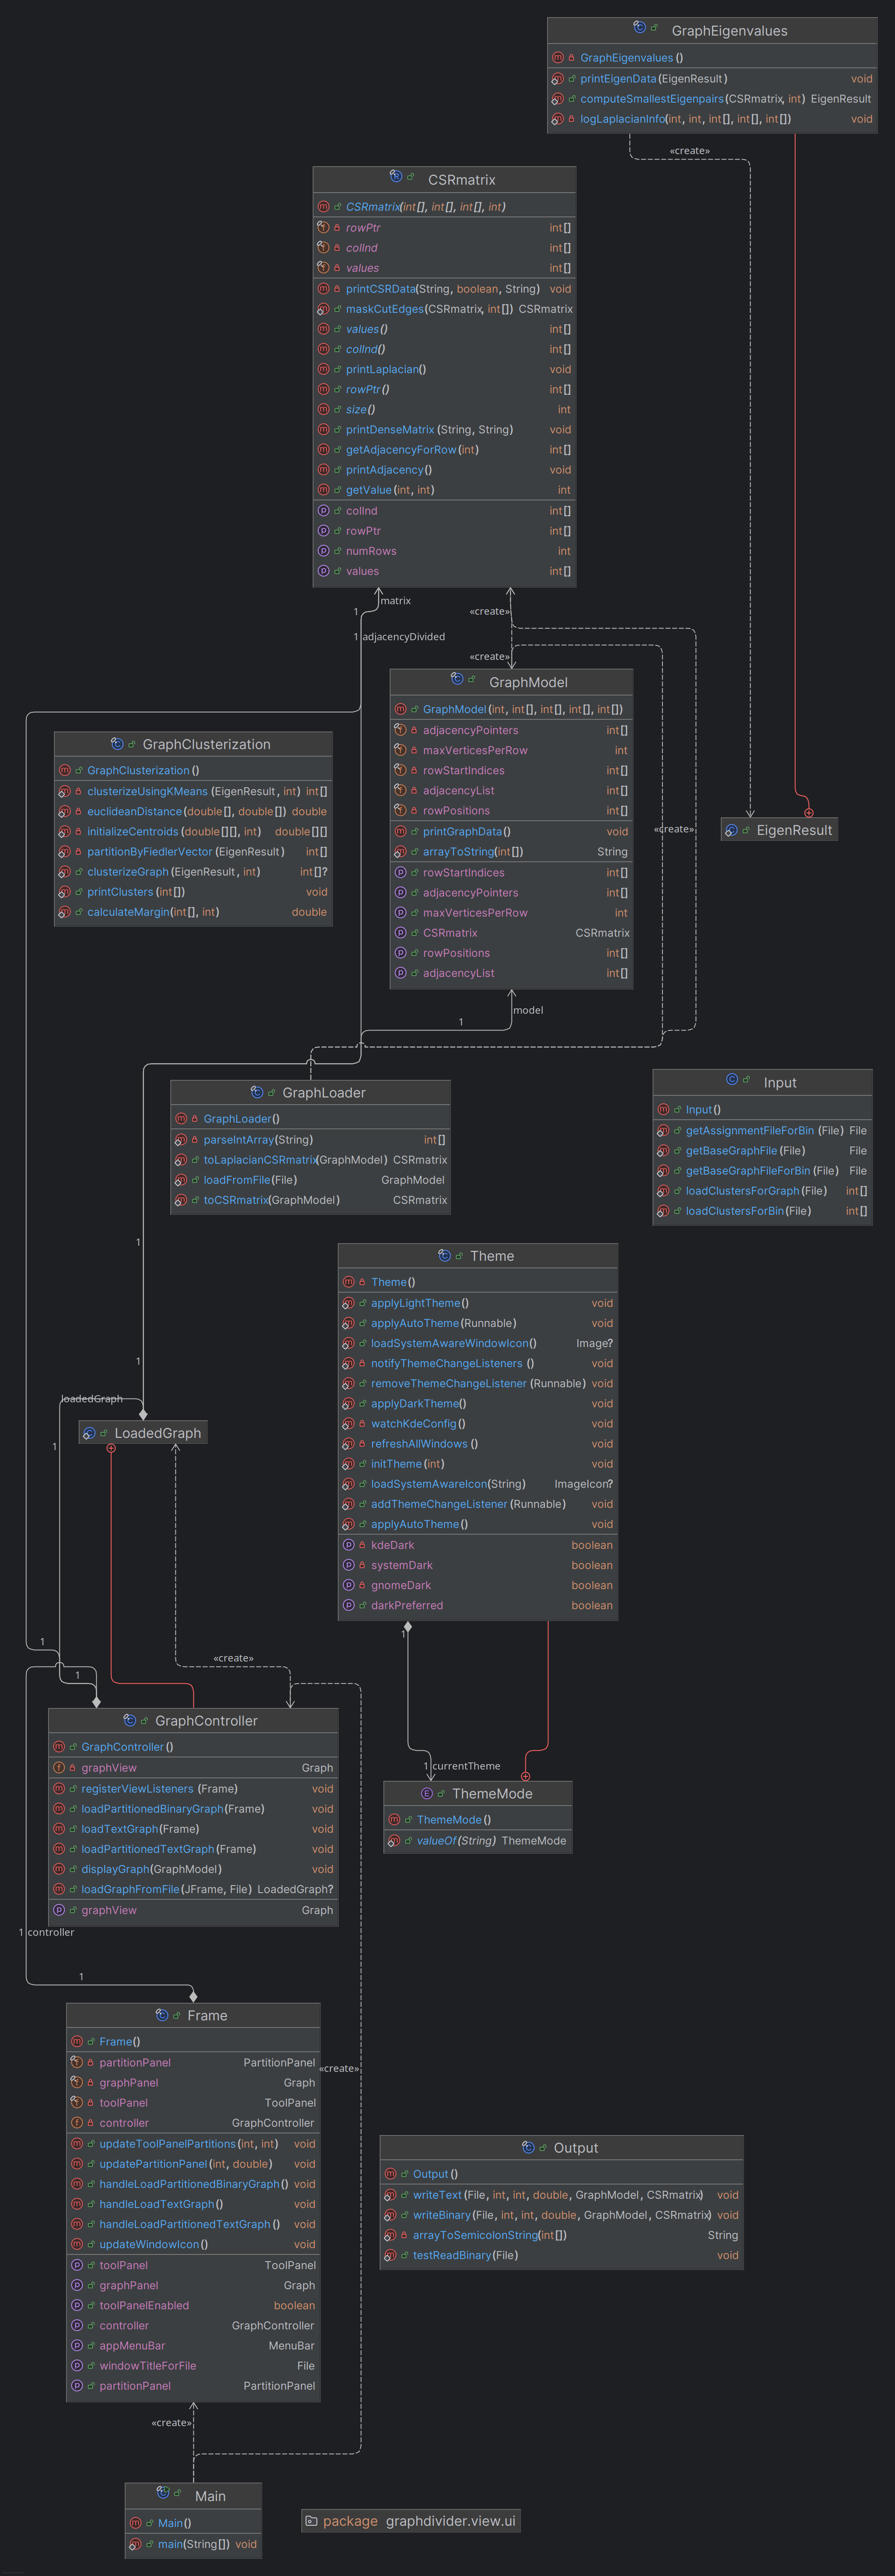
\includegraphics[width=0.45\linewidth]{img/UML.png}
        \caption{Diagram klas UML}
        \label{fig:uml}
    \end{figure}



\section{Najważniejsze klasy i funkcje w programie}

    \begin{enumerate}
        \item \textbf{Frame} \\
        Klasa \texttt{graphdivider.view.Frame} odpowiada za główne okno aplikacji oraz integrację wszystkich paneli interfejsu użytkownika. Zarządza panelem narzędzi (\texttt{ToolPanel}), panelem podziału (\texttt{PartitionPanel}), panelem wizualizacji grafu (\texttt{Graph}) oraz paskiem menu (\texttt{MenuBar}). Udostępnia metody do aktualizacji interfejsu, obsługi zdarzeń oraz przekazywania poleceń do kontrolera.

        \begin{figure}[H]
            \centering
            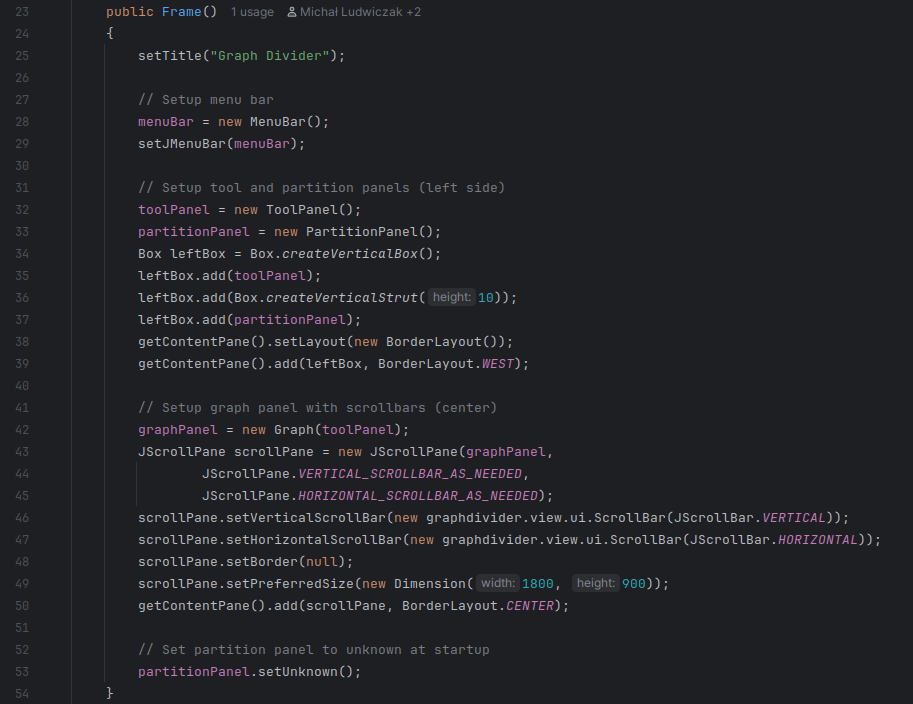
\includegraphics[width=1\linewidth]{img/frame.png}
            \caption{Konstruktor klasy Frame}
            \label{fig:frame}
        \end{figure}
    
        \item \textbf{GraphController} \\
        Klasa \texttt{graphdivider.controller.GraphController} pełni rolę kontrolera w architekturze MVC. Odpowiada za obsługę logiki aplikacji: ładowanie grafów z plików, inicjalizację modelu, wywoływanie algorytmów podziału oraz aktualizację widoku. Rejestruje nasłuchiwacze zdarzeń dla interfejsu użytkownika i zarządza przepływem danych pomiędzy modelem a widokiem.

        \begin{figure}[H]
            \centering
            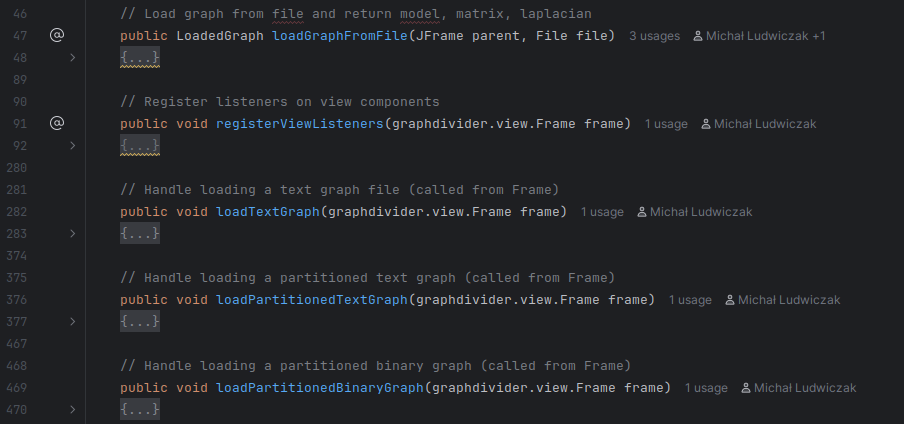
\includegraphics[width=1\linewidth]{img/graphcontroller.png}
            \caption{Interfejsy funkcji kontrolujących wczytywanie plików wejściowych (GraphController)}
            \label{fig:graphcontroller}
        \end{figure}
    
        \item \textbf{GraphEigenvalues} \\
        Klasa \texttt{graphdivider.model.GraphEigenvalues} realizuje obliczanie wartości i wektorów własnych macierzy Laplace'a grafu. Kluczowa metoda \texttt{computeSmallestEigenpairs} wykorzystuje bibliotekę ARPACK do wydajnych obliczeń spektralnych, zwracając obiekt \texttt{EigenResult} z tablicą wartości własnych i odpowiadającymi im wektorami własnymi.

        \begin{figure}[H]
            \centering
            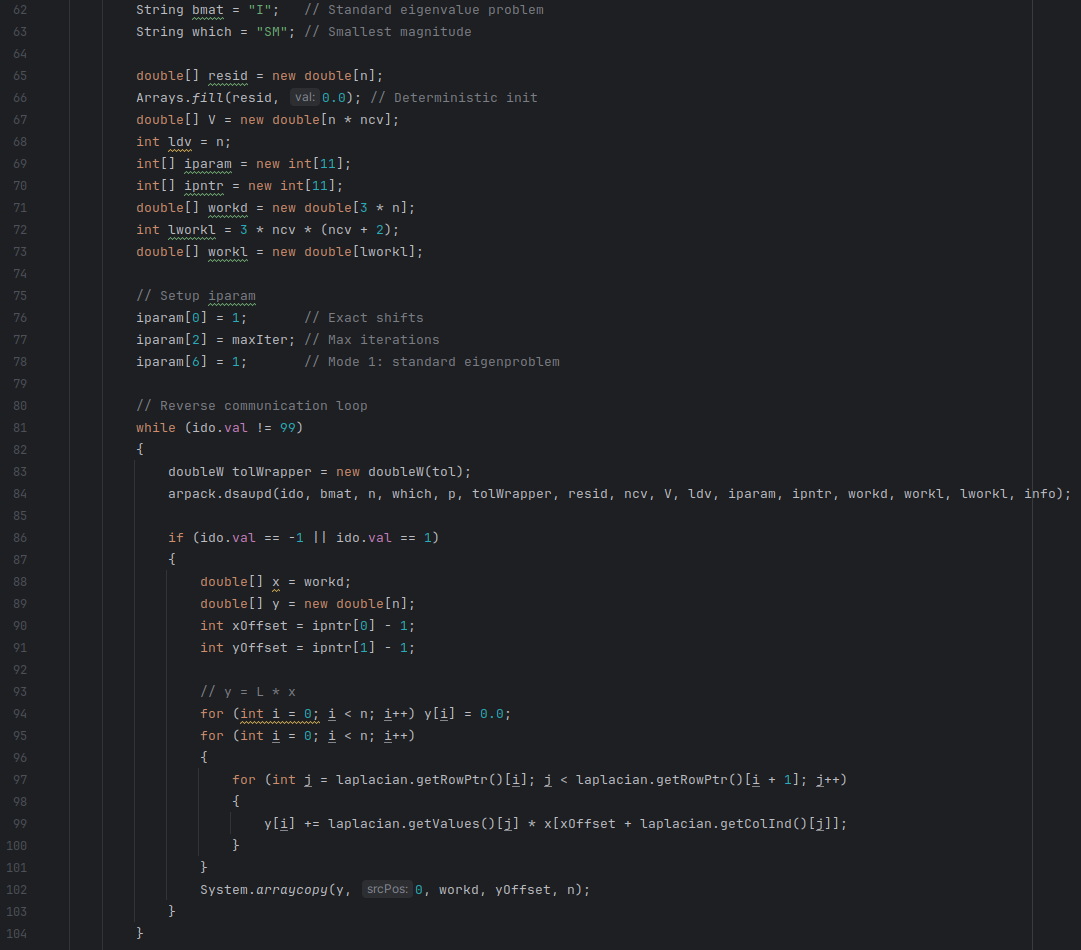
\includegraphics[width=1\linewidth]{img/eigenvalues.png}
            \caption{Fragment funkcji computeSmallestEigenpairs (argumenty + główna pętla, bez normalizacji)}
            \label{fig:eigenvalues}
        \end{figure}
    
        \item \textbf{GraphClusterization} \\
        Klasa \texttt{graphdivider.model.GraphClusterization} odpowiada za podział grafu na części na podstawie wyników analizy spektralnej. Udostępnia metody do podziału według wektora Fiedlera (dla dwóch części) oraz zbalansowanego klasteryzowania k-średnich (dla większej liczby części). Zawiera także funkcje pomocnicze do obliczania marginesu i wypisywania wyników podziału.

        \begin{figure}[H]
            \centering
            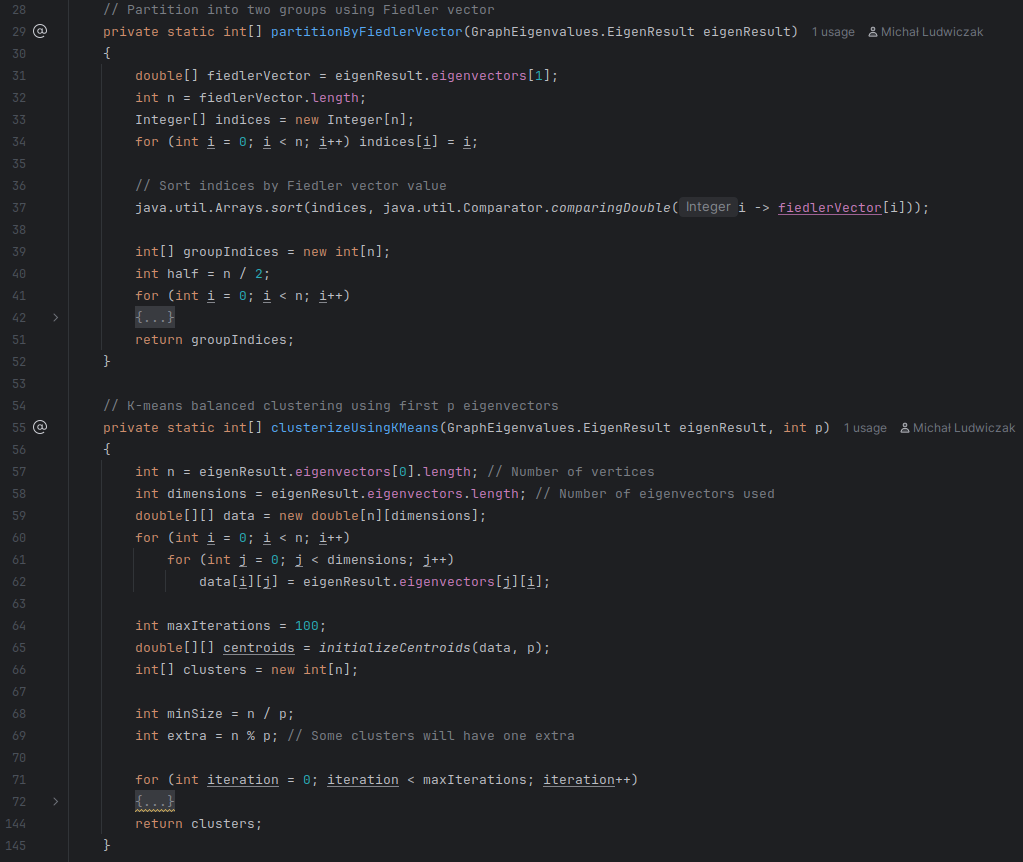
\includegraphics[width=1\linewidth]{img/clusterization.png}
            \caption{Funkcje odpowiadające za dzielenie grafu na podstawie obliczonych wartości wektorów własnych (względem wektora Fiedlera + zbalansowana klasteryzacja k-średnich}
            \label{fig:enter-label}
        \end{figure}
    
        \item \textbf{Graph} \\
        Klasa \texttt{graphdivider.view.ui.Graph} odpowiada za wizualizację grafu w interfejsie graficznym. Pozwala na rysowanie wierzchołków i krawędzi, aktualizację kolorowania wierzchołków według przypisanych części oraz dynamiczne odświeżanie widoku po podziale grafu.
        
        \begin{figure}[H]
            \centering
            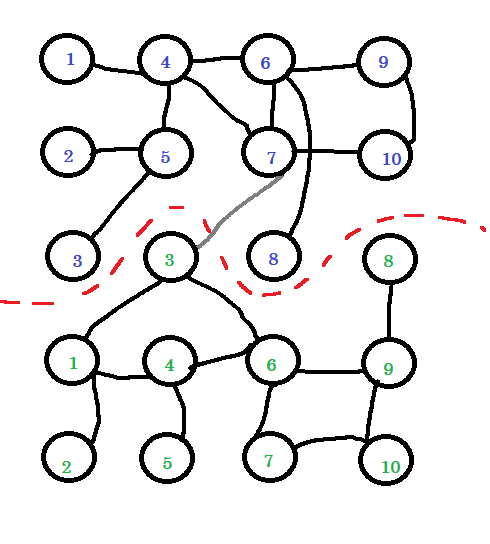
\includegraphics[width=1\linewidth]{img/Graph.png}
            \caption{Fragment klasy Graph, funkcja displayGraph do wyświetlania grafu w panelu}
            \label{fig:Graph}
        \end{figure}
        
    \end{enumerate}
        


\section{Pliki wejściowe i wyjściowe dla trybu dzielenia}

    \subsection{Plik wejściowy (\texttt{.csrrg})}
    
        Format pliku składa się z pięciu sekcji zapisanych w kolejnych liniach:
        \begin{enumerate}
            \item Maksymalna liczba wierzchołków w dowolnym wierszu macierzy sąsiedztwa.
            \item Lista sąsiadów wszystkich wierzchołków zapisana sekwencyjnie.
            \item Wskaźniki (indeksy) na początki list sąsiedztwa dla poszczególnych wierzchołków.
            \item Lista grup wierzchołków połączonych krawędziami (reprezentacja krawędzi).
            \item Wskaźniki na początki grup węzłów z poprzedniej listy.
        \end{enumerate}

        \begin{figure}[H]
            \centering
            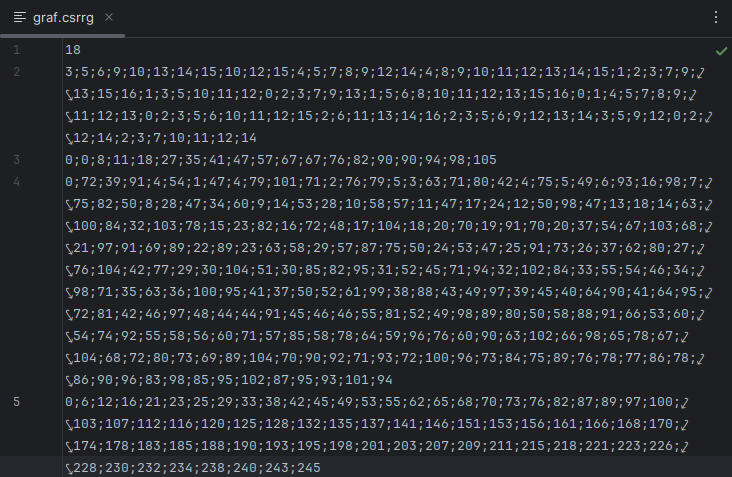
\includegraphics[width=1\linewidth]{img/input_csrrg.png}
            \caption{Przykładowy plik wejściowy (graph.csrrg)}
            \label{fig:input_csrrg}
        \end{figure}
    
    \subsection{Plik wyjściowy (\texttt{.csrrg2} / \texttt{.bin})}

    Po przetworzeniu danych program generuje plik wyjściowy w jednym z dwóch formatów:
    \begin{itemize}
        \item \texttt{.csrrg2} — tekstowa forma pliku wyjściowego, wzorowana na formacie wejściowym .csrrg, ale zawierająca dodatkową linię nagłówkową z wynikiem działania programu.
        \item \texttt{.bin} — binarna wersja pliku tekstowego \texttt{.csrrg2}.
    \end{itemize}
    
    W pierwszej linii pliku wyjściowego zapisywany jest rezultat działania programu w formacie:
    \begin{center}
    \texttt{<liczba\_części> <liczba\_przecięć> <zachowany\_margines>}
    \end{center}
    Przykład:
    \begin{center}
    \texttt{3 14026 0,00}
    \end{center}

    \begin{figure}[H]
        \centering
        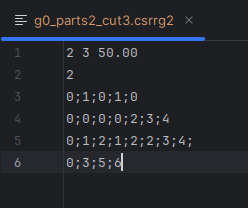
\includegraphics[width=0.75\linewidth]{img/output.png}
        \caption{Przykładowy plik wyjściowy o domyślnej nazwie \texttt{g0\_parts2\_cut3.csrrg2}, powstały w wyniku podziału grafu \texttt{g0.csrrg} na 2 części z przecięciem 3 krawędzi}
        \label{fig:output}
    \end{figure}

    


\section{Pliki wejściowe dla trybu wyświetlenia podzielonego grafu}
    (pliki wyjściowe programu w C)

    \subsection{Plik wejściowy w formacie \texttt{.csrrg}}
    Plik przyjmuje postać taką jak plik wejściowy w formacie .csrrg z tym, że linijki po 5 linijce zawierają wierzchołki należące do danych kolejnych podgrup.
    \begin{figure}[H]
        \centering
        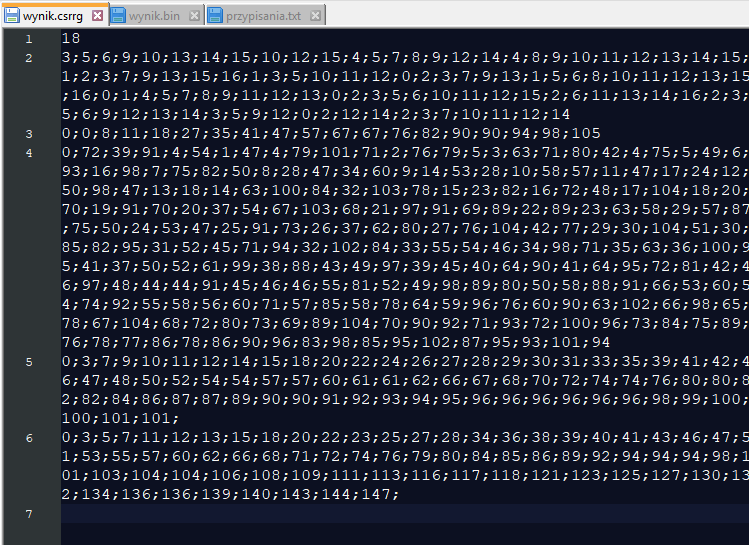
\includegraphics[width=0.9\linewidth]{img/plik_c.png}
        \caption{Przykładowy plik wejściowy dla trybu wyświetlenia}
        \label{fig:plik_c}
    \end{figure}

    \subsection{Plik wejściowy w formacie binarnym (\texttt{.bin})}
    Zapis taki sam jak w formacie .csrrg, ale w formacie binarnym z wypisaniem ilości elementów w linijkach.



\section{Obsługa błędów i wyjątków}

    W aplikacji zaimplementowano obsługę najważniejszych błędów i wyjątków, które mogą wystąpić podczas pracy programu. Dzięki temu użytkownik otrzymuje czytelne komunikaty o problemach, a aplikacja nie kończy działania w sposób niekontrolowany.
    
    \begin{itemize}
        \item \textbf{Błędy podczas wczytywania plików} \\
        Podczas próby wczytania grafu z pliku tekstowego lub binarnego obsługiwane są wyjątki związane z brakiem pliku, błędnym formatem lub błędami wejścia/wyjścia (\texttt{IOException}). W przypadku wykrycia błędu użytkownik otrzymuje komunikat w oknie dialogowym, a operacja jest przerywana.
    
        \item \textbf{Nieprawidłowe dane wejściowe} \\
        Program sprawdza poprawność parametrów podziału grafu (liczba części, margines). Jeżeli użytkownik wprowadzi nieprawidłowe wartości (np. liczbę części większą niż liczba wierzchołków, margines spoza zakresu), wyświetlany jest komunikat o błędzie i operacja nie jest wykonywana.
    
        \item \textbf{Błędy podczas obliczeń spektralnych} \\
        Podczas obliczania wartości własnych i wektorów własnych macierzy Laplace'a mogą wystąpić wyjątki związane z nieprawidłową macierzą lub brakiem zbieżności algorytmu ARPACK. Takie wyjątki są przechwytywane, a użytkownik informowany jest o niepowodzeniu operacji.
    
        \item \textbf{Błędy podczas zapisu wyników} \\
        W przypadku problemów z zapisem wyników do pliku (np. brak uprawnień, błąd dysku) obsługiwane są wyjątki wejścia/wyjścia. Użytkownik otrzymuje stosowny komunikat, a program nie kończy działania.
    
        \item \textbf{Błędy podczas wizualizacji} \\
        Jeżeli podczas rysowania grafu lub aktualizacji widoku wystąpi błąd (np. brak danych do wyświetlenia), aplikacja wyświetla komunikat i nie próbuje wykonać niepoprawnej operacji.
    \end{itemize}
    
    Wszystkie powyższe sytuacje są obsługiwane w kodzie poprzez instrukcje \texttt{try-catch}, a użytkownik jest informowany o problemach za pomocą okien dialogowych lub komunikatów w interfejsie graficznym.
    



\section{Przykłady użycia}

    \subsection{Wczytywanie grafu z pliku tekstowego}
    
    Aby wczytać graf z pliku tekstowego (np. \texttt{src/main/resources/graphs/graf.csrrg}), wybierz opcję \texttt{Load File -> Graph (Text)...} z paska menu. Program odczyta dane grafu w formacie CSR i wyświetli jego strukturę w głównym obszarze aplikacji.
    
    \subsection{Podział grafu na \texttt{x} części z marginesem \texttt{y\%}}
    
    Po załadowaniu grafu ustaw w panelu narzędziowym liczbę części (\texttt{x}) oraz margines tolerancji wielkości części (\texttt{y\%}). Następnie kliknij przycisk \texttt{Divide Graph}. Program dokona podziału grafu na \texttt{x} części, minimalizując liczbę przeciętych krawędzi i zachowując zadany margines liczebności wierzchołków w każdej części.
    
    \subsection{Zapisanie wyniku do pliku tekstowego}
    
    Po zakończeniu podziału wybierz opcję \texttt{Save File -> Partitioned Graph (Text)...} z menu. Wynik zostanie zapisany w katalogu \texttt{src/main/resources/divided\_graphs/} w formacie \texttt{.csrrg2}, zawierającym dodatkową linię nagłówkową z informacją o wyniku działania programu oraz przypisania wierzchołków do części.
    
    \subsection{Zapisanie wyniku do pliku binarnego}
    
    Aby zapisać wynik w formacie binarnym, wybierz opcję \texttt{ZSave File -> Partitioned Graph (Binary} z menu. Plik zostanie zapisany w katalogu \texttt{src/main/resources/divided\_graphs/} z rozszerzeniem \texttt{.bin}, co umożliwia szybkie wczytanie podzielonego grafu w przyszłości.
    
    \subsection{Przykładowe pliki}
    


\section{Wymagania niefunkcjonalne}

    Poniżej przedstawiono kluczowe wymagania niefunkcjonalne dla aplikacji:
    
    \begin{itemize}
        \item \textbf{Wydajność:} Czas podziału grafu powinien być jak najkrótszy dla danej wielkości grafu. Dla grafów zawierających do 1000 wierzchołków, czas przetwarzania nie powinien przekraczać minuty na standardowym sprzęcie klasy PC.
        \item \textbf{Użyteczność:} Interfejs użytkownika powinien być intuicyjny i zgodny z ogólnie przyjętymi standardami projektowania GUI.
        \item \textbf{Skalowalność:} Aplikacja powinna umożliwiać obsługę grafów o różnej wielkości, od małych do dużych.
        \item \textbf{Przenośność:} Aplikacja powinna działać poprawnie na różnych systemach operacyjnych wspierających środowisko Java.
        \item \textbf{Utrzymywalność:} Kod źródłowy aplikacji powinien być czytelny i dobrze udokumentowany, aby ułatwić przyszłe modyfikacje i rozwój.
    \end{itemize}



\section{Podsumowanie}

    Program umożliwia szybki i efektywny podział grafów dzięki wykorzystaniu biblioteki ARPACK, która pozwala na błyskawiczne obliczanie najmniejszych par własnych macierzy Laplace'a nawet dla bardzo dużych grafów. Zastosowanie zbalansowanej klasteryzacji k-średnich (k-means) sprawia, że margines nierówności podziału jest minimalny, co przekłada się na wysoką jakość wyników. Intuicyjny interfejs graficzny umożliwia łatwe wprowadzanie parametrów podziału oraz dynamiczne dostosowywanie zakresów kontrolek w zależności od wczytanego grafu. Wizualizacja grafu jest czytelna i pozwala na szybkie rozróżnienie poszczególnych części dzięki kolorowaniu wierzchołków według przypisania do części. Całość rozwiązania zapewnia wysoką wydajność, wygodę użytkowania oraz przejrzystość prezentowanych wyników.

    

\begin{thebibliography}{9}

\bibitem{youtube_video}
Leonid Zhukov, \textit{Lecture 7. Graph partitioning algorithms.}, YouTube, 24 luty 2021, Dostępny na 11 maja 2025 w: \url{https://youtu.be/zZae_C2BU_4}

\bibitem{laplacian_matrix}
\textit{Laplacian matrix}, Wikipedia, Dostępne na 11 maja 2025 w: \url{https://en.wikipedia.org/wiki/Laplacian_matrix}

\bibitem{k-means}
\textit{Algorytm centroidów}, Wikipedia, Dostępne na 11 maja 2025 w:
\url{https://pl.wikipedia.org/wiki/Algorytm_centroid%C3%B3w}

\end{thebibliography}


\end{document}
